
\documentclass[12pt, reqno, oneside]{amsart}
\usepackage{geometry} % see geometry.pdf on how to lay out the page. There's lots.
\geometry{a4paper} % or letter or a5paper or ... etc
% \geometry{landscape} % rotated page geometry
 \usepackage{graphicx}  %  incorporate images into your LaTeX document
% To show syntax format of c programming code 
\usepackage{minted}
% make a clickable Table of Contents
\usepackage{hyperref}
\hypersetup{
    colorlinks=true, %set true if you want colored links
    linktoc=all,     %set to all if you want both sections and subsections linked
    linkcolor=blue,  %choose some color if you want links to stand out
}

% use the quote environment inside by \begin{framed} \end{framed}
\usepackage{framed}
% display the day of the week
\usepackage{datetime}

% Hide subsection in table of content
\setcounter{tocdepth}{1}

% See the ``Article customise'' template for come common customisations

\title{Interview Questions}
\author{Yuanming Yu}
\date{\today}  % delete this line to display the current date

%%% BEGIN DOCUMENT
\begin{document}

\maketitle
\tableofcontents

% hide all subsection from now on
\addtocontents{toc}{\protect\setcounter{tocdepth}{1}}

\section{Splitting Linked List}
\begin{framed}
\begin{quote}
Given a list, split it into two sublists — one for the front half, and one for the back half. If the number of elements is odd, the extra element should go in the front list. So FrontBackSplit() on the list {2, 3, 5, 7, 11} should yield the two lists {2, 3, 5} and {7, 11}.
\end{quote}
\end{framed}

This is a very good linked list question, as there are tricky cases you have to consider, and getting them all right in one place is harder than it looks. It also has a very obvious simple solution, which is to iterate the list twice. The first time to count how many elements in the list, and the second time to find the splitting point.

Can we do better? You bet.

Hint: Try to use two pointers to traverse the list.

\subsection{Solution}
We use two pointers (we call it a slow pointer and a fast pointer). The slow pointer advances one node at a time, while the fast pointer advances two nodes at a time. By the time the fast pointer reaches the end, the slow pointer would have reached the splitting point (or near). Care must be taken to account those special cases. Below is a solution that works for all cases.

\begin{minted}[mathescape,
               linenos,
               numbersep=5pt,
               fontsize=\footnotesize,
               frame=lines,
               framesep=2mm]{cpp}
               
void FrontBackSplit(Node *head, Node **front, Node **back) {
  if (!head) return;  // Handle empty list
  Node *front_last_node;
  Node *slow = head;
  Node *fast = head;
  while (fast) {
    front_last_node = slow;
    slow = slow->next;
    fast = (fast->next) ? fast->next->next : NULL;
  }
  front_last_node->next = NULL;  // ends the front sublist
  *front = head;
  *back = slow;
}
\end{minted}


\section{Insert into a Cyclic Sorted List}
\begin{framed}
\begin{quotation}
Given a node from a cyclic linked list which has been sorted, write a function to insert a value into the list such that it remains a cyclic sorted list. The given node can be any single node in the list.
\end{quotation}
\end{framed}

First, it is important that you understand what a cyclic linked list is. A cyclic linked list differs from a normal linked list in that its tail node points back to its head node instead of NULL.

This problem seems a little tricky because the given node is not necessarily the list’s head (ie, the node that has the smallest element). It shouldn’t take you too long to come up with an idea, but beware. There are hidden traps around the corner and you are bound to make some mistakes if you are not careful in your thoughts.

\begin{figure}[htbp] %  figure placement: here, top, bottom, or page
   \centering
   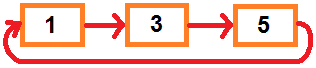
\includegraphics[width=3in]{figs/cyclic_list1.png} 
   \caption{A cyclic sorted linked list.}
   \label{fig:cyclic_list1}
\end{figure}

Note that the tail is pointing back to its head. The only reference to the list is a given node which can be any node in the list. Let’s say that you need to insert 4 into the list.

\begin{figure}[htbp] %  figure placement: here, top, bottom, or page
   \centering
   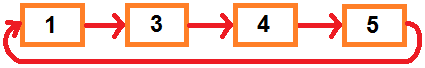
\includegraphics[width=4in]{figs/cyclic_list2.png} 
   \caption{This is how the cyclic list becomes after inserting 4. Note that the cyclic linked list remained in sorted order.}
   \label{fig:cyclic_list1}
\end{figure}

\subsection{Hint}
It is best to list all kinds of cases first before you jump into coding. Then, it is much easier to reduce the number of cases your code need to handle by combining some of them into a more generic case. Try to also list down all possible edge cases if you have time. You might discover a bug before you even start coding!

\subsection{Solution}
Basically, you would have a loop that traverse the cyclic sorted list and find the point where you insert the value (Let’s assume the value being inserted called x). You would only need to consider the following three cases:

\begin{framed}
\begin{quotation}
\begin{itemize}
\item $prev \rightarrow val \leq x \leq current \rightarrow val$:
Insert between prev and current.
\item $x$ is the maximum or minimum value in the list:
Insert before the head. (ie, the head has the smallest value and its $prev \rightarrow val > head \rightarrow val)$.
\item 
Traverses back to the starting point:
Insert before the starting point.
\end{itemize}
\end{quotation}
\end{framed}

\begin{minted}[mathescape,
               linenos,
               numbersep=5pt,
               fontsize=\footnotesize,
               frame=lines,
			   tabsize=4,
               framesep=2mm]{cpp}

void insert(Node *& aNode, int x) {
  if (!aNode) {
    aNode = new Node(x);
    aNode->next = aNode;
    return;
  }

  Node *p = aNode;
  Node *prev = NULL;
  do {
    prev = p;
    p = p->next;
    if (x <= p->data && x >= prev->data) break;   // For case 1)
    if ((prev->data > p->data) && (x < p->data || x > prev->data)) break; // For case 2)
  } while (p != aNode);   // when back to starting point, then stop. For case 3)

  Node *newNode = new Node(x);
  newNode->next = p;
  prev->next = newNode;
}

\end{minted}



\section{Detecting a Loop in a Singly Linked List}

\begin{framed}
\begin{quotation}
Given a singly linked list, find if there exist a loop.
\end{quotation}
\end{framed}

This is one of the most common interview questions asked during a technical interview. I call it the classic linked list question.

The naive approach requires $O(N^2)$ time and $O(N)$ space. Basically you store all visited nodes, and compare each of them while traversing each node.

\subsection{Solution}
The best solution runs in $O(N)$ time and uses $O(1)$ space. It uses two pointers (one slow pointer and one fast pointer). The slow pointer advances one node at a time, while the fast pointer traverses twice as fast. If the list has loop in it, eventually the fast and slow pointer will meet at the same node. On the other hand, if the loop has no loop, the fast pointer will reach the end of list before the slow pointer does.

\begin{minted}[mathescape,
               linenos,
               numbersep=5pt,
               fontsize=\footnotesize,
               frame=lines,
			   tabsize=4,
               framesep=2mm]{cpp}

bool hasLoop(Node *head) {
  Node *slow = head, *fast = head;
  while (slow && fast && fast->next) {
    slow = slow->next;
    fast = fast->next->next;
    if (slow == fast)
      return true;
  }
  return false;
}
\end{minted}


\subsection{Alternative solutions}
There is another alternative solution that also runs in $O(N)$ time and $O(1)$ space, but the catch is it requires modification to the list. Try reversing the list if it has a loop in it. What do you see? Yes, eventually you will arrive back at the beginning (the head node). Read next post here on how to reverse a linked list iteratively and recursively.

Here are some very common questions on linked list from easy to difficult, all available at supply \textbf{LinkedListProblems.pdf}. Highly recommended!


\section{Reversing linked list iteratively and recursively}
\begin{framed}
\begin{quote}
Implement the reversal of a singly linked list iteratively and recursively.
\end{quote}
\end{framed}

Reversing linked list can be done both iteratively and recursively. In my opinion, the iterative solution should be more efficient and less memory overhead than its recursive counterpart (Imagine reversing a link list that has one million elements recursively! It would quickly run out of stack space).

The recursive solution can be coded in fewer lines of code, but is harder to code correctly. On the other hand, the iterative solution requires more code but is easier to verify.

\subsection{Solution}
1) The iterative way:
\begin{minted}[mathescape,
               linenos,
               numbersep=5pt,
               fontsize=\footnotesize,
               frame=lines,
               framesep=2mm]{cpp}
               
void reverse(Node*& head) {
  if (!head) return;
  Node* prev = NULL;
  Node* curr = head;
  while (curr) {
    Node* next = curr->next;
    curr->next = prev;
    prev = curr;
    curr = next;
  }
  head = prev;
}
\end{minted}


Please do note that the head pointer is passed in by reference. If you have trouble understanding the syntax, think the pointer as a type, and an \& sign followed by a type signifies the variable is passed by reference. The head pointer must be passed in by reference whenever there might be a change to the head pointer itself!\newline

2) The recursive way:
\begin{minted}[mathescape,
               linenos,
               numbersep=5pt,
               fontsize=\footnotesize,
               frame=lines,
               framesep=2mm]{cpp}
               
void reverse(Node*& p) {
  if (!p) return;
  Node* rest = p->next;
  if (!rest) return;
  reverse(rest);
  p->next->next = p;
  p->next = NULL;
  p = rest;
}
\end{minted}

Can you see why the head pointer is eventually updated to point to the last element of the list? Try to draw a diagram and see how the rest pointer changes when the recursion exits. (Hint: the rest pointer points to the last element and does not change).


\section{Convert Sorted List to Balanced Binary Search Tree }
\begin{framed}
\begin{quotation}
Given a singly linked list where elements are sorted in ascending order, convert it to a height balanced BST.
\end{quotation}
\end{framed}

\begin{figure}[htbp] %  figure placement: here, top, bottom, or page
   \centering
   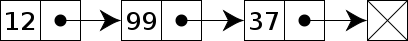
\includegraphics[width=4in]{figs/Singly-linked-list.png} 
   \caption{Singly-linked lists contain nodes which have a data field as well as a \textit{next} field, which points to the next node in the linked list.}
   \label{fig:Singly-linked-list}
\end{figure}

\subsection{Hint}
How about inserting nodes following the list’s order? If we can achieve this, we no longer need to find the middle element, as we are able to traverse the list while inserting nodes to the tree.

\subsection{Best Solution}
As usual, the best solution requires you to think from another perspective. In other words, we no longer create nodes in the tree using the top-down approach. We create nodes bottom-up, and assign them to its parents. The bottom-up approach enables us to access the list in its order while creating nodes.

Isn’t the bottom-up approach neat? Each time you are stucked with the top-down approach, give bottom-up a try. Although bottom-up approach is not the most natural way we think, it is extremely helpful in some cases. However, you should prefer top-down instead of bottom-up in general, since the latter is more difficult to verify in correctness.

Below is the code for converting a singly linked list to a balanced BST. Please note that the algorithm requires the list’s length to be passed in as the function’s parameters. The list’s length could be found in $O(N)$ time by traversing the entire list’s once. The recursive calls traverse the list and create tree’s nodes by the list’s order, which also takes $O(N)$ time. Therefore, the overall run time complexity is still $O(N)$.

\begin{minted}[mathescape,
               linenos,
               numbersep=5pt,
               fontsize=\footnotesize,
               frame=lines,
			   tabsize=4,
               framesep=2mm]{cpp}

BinaryTree* sortedListToBST(ListNode *& list, int start, int end) {
  if (start > end) return NULL;
  // same as (start+end)/2, avoids overflow
  int mid = start + (end - start) / 2;
  BinaryTree *leftChild = sortedListToBST(list, start, mid-1);
  BinaryTree *parent = new BinaryTree(list->data);
  parent->left = leftChild;
  list = list->next;
  parent->right = sortedListToBST(list, mid+1, end);
  return parent;
}
 
BinaryTree* sortedListToBST(ListNode *head, int n) {
  return sortedListToBST(head, 0, n-1);
}
\end{minted}



\section{A Distance Maximizing Problem}
Given an array $A$ of integers, find the maximum of $j-i$ subjected to the constraint of $A[i] < A[j]$.
\subsection{Best Solution $O(N)$}

\begin{figure}[htbp] %  figure placement: here, top, bottom, or page
   \centering
   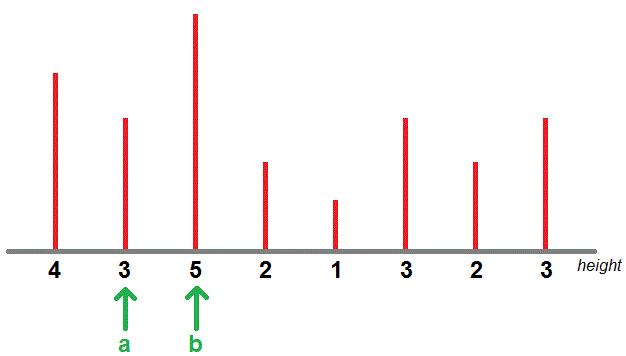
\includegraphics[width=4in]{figs/A_Distance_Maximizing_Problem.png} 
   \caption{Given two indices a and b, where would you rather choose as a potential starting point?}
   \label{fig:dist_max}
\end{figure}

Assume that choosing index b as the starting point, the max distance is j-b, where $A[j] > A[b]$. Now, since $a < b$ and $A[a]$ is not taller than $A[b]$ which implies that $A[j] > A[a]$, we can form a farther distance by choosing a as the starting index. Therefore, we cannot choose b as the starting point as this forms a contradiction.

Generally, we want to choose only starting points with no such lines that are shorter to its left side. From the diagram above, only lines of index 0, 1, 3, 4 are valid starting points.

Once we gather all valid starting points by scanning once from left to right, we are able to obtain the maximum distance by scanning backwards.

It is obvious that if the ending point is less than the shortest starting point, then it won’t be a valid solution for all other starting points. Therefore, we scan from right to left until we meet the first ending point that satisfies the condition. Then, we proceed to the next shortest starting point, and continue on from the previous ending point. Using this strategy, we would guarantee that we are able to find the maximum distance in $O(N)$ running time.

\section{Find the $k$-th Smallest Element in the Union of Two Sorted Arrays}
Given two sorted arrays $A$, $B$ of size m and n respectively. Find the $k$-th smallest element in the union of $A$ and $B$. You can assume that there are no duplicate elements.
\subsection{The best solution, but non-trivial, $O(\log m + \log n)$}

We try to approach this tricky problem by comparing middle elements of $A$ and $B$, which we identify as $A_{i}$ and $B_{j}$. If $A_{i}$ is between $B_{j}$ and $B_{j-1}$, we have just found the $i+j+1$ smallest element. Why? Therefore, if we choose i and j such that $i+j = k-1$, we are able to find the $k$-th smallest element. This is an important invariant that we must maintain for the correctness of this algorithm.

\begin{framed}
\begin{quote}
Maintaining the invariant
$$i + j = k - 1$$
If $B_{j-1} < A_{i} < B_{j}$, then $A_{i}$ must be the $k$-th smallest, \newline
or else if $A_{i-1} < B_{j} < A_{i}$, then $B_{j}$ must be the $k$-th smallest.
\end{quote}
\end{framed}

Using the above relationship, it becomes clear that when $A_{i} < B_{j}$, $A_{i}$ and its lower portion could never be the $k$-th smallest element. So do $B_{j}$ and its upper portion. Therefore, we could conveniently discard $A_{i}$ with its lower portion and $B_{j}$ with its upper portion.

On the other hand, the case for $A_{i} > B_{j}$ is just the other way around. Easy.

\begin{minted}[mathescape,
               linenos,
               numbersep=5pt,
               fontsize=\footnotesize,
               frame=lines,
               framesep=2mm]{cpp}
int findKthSmallest(int A[], int m, int B[], int n, int k) {
  assert(m >= 0); assert(n >= 0); assert(k > 0); assert(k <= m+n);
  
  int i = (int)((double)m / (m+n) * (k-1));
  int j = (k-1) - i;
 
  assert(i >= 0); assert(j >= 0); assert(i <= m); assert(j <= n);
  // invariant: i + j = k-1
  // Note: A[-1] = -INF and A[m] = +INF to maintain invariant
  int Ai_1 = ((i == 0) ? INT_MIN : A[i-1]);
  int Bj_1 = ((j == 0) ? INT_MIN : B[j-1]);
  int Ai   = ((i == m) ? INT_MAX : A[i]);
  int Bj   = ((j == n) ? INT_MAX : B[j]);
 
  if (Bj_1 < Ai && Ai < Bj)
    return Ai;
  else if (Ai_1 < Bj && Bj < Ai)
    return Bj;
 
  assert((Ai > Bj && Ai_1 > Bj) || 
         (Ai < Bj && Ai < Bj_1));
 
  // if none of the cases above, then it is either:
  if (Ai < Bj)
    // exclude Ai and below portion
    // exclude Bj and above portion
    return findKthSmallest(A+i+1, m-i-1, B, j, k-i-1);
  else /* Bj < Ai */
    // exclude Ai and above portion
    // exclude Bj and below portion
    return findKthSmallest(A, i, B+j+1, n-j-1, k-j-1);
}
\end{minted}


\section{Reverse a number}
Given a unsigned int number, how to reverse it?
\subsection{Solution in $O(\log n)$}
The  $O(n)$ method is easy, we hope to do it faster.
Swap the odd and even position, and then swap every two-length position and its next, and so on…

Example:
\begin{verbatim}
(10010010)
(1 0 0 1 0 0 1 0) -> (0 1 1 0 0 0 0 1)
(01 10 00 01) -> (10 01 01 00)
(1001 0100) -> (0100 1001)
(01001001)
\end{verbatim}

Here goes the  $O(\log n)$way:
\begin{minted}[mathescape,
               linenos,
               numbersep=5pt,
               fontsize=\footnotesize,
               frame=lines,
			   tabsize=4,
               framesep=2mm]{cpp}
typedef unsigned int uint;

uint reverse(uint x) {
	// Assume it is on 32-bits operating system.
	// It's also easy to generalize to other platform
	assert (sizeof(x) == 4);
	// 0xA = (1010), 0x5 = (0101), 0xC = (1100), 0x3 = (0011) ...
	x = ((x & 0xAAAAAAAA)>>1) | ((x & 0x55555555)<<1);
	x = ((x & 0xCCCCCCCC)>>2) | ((x & 0x33333333)<<2);
	x = ((x & 0xF0F0F0F0)>>4) | ((x & 0x0F0F0F0F)<<4);
	x = ((x & 0xFF00FF00)>>8) | ((x & 0x00FF00FF)<<8);
	x = ((x & 0xFFFF0000)>>16) | ((x & 0x0000FFFF)<<16);
	return x;
}               
\end{minted}



\addtocontents{toc}{\protect\setcounter{tocdepth}{2}}
%from now on subsections are shown like usual

\section{Tips on Interviews}

\subsection{Hiring: The Lake Wobegon Strategy}
\textit{Posted 12th March 2006 by Peter Norvig, Director, Google Research}

You know the Google story: small start-up of highly-skilled programmers in a garage grows into a large international company. But how do you maintain the skill level while roughly doubling in size each year? We rely on the Lake Wobegon Strategy, which says \textbf{only hire candidates who are above the mean of your current employees}. An alternative strategy (popular in the dot-com boom period) is to justify a hire by saying "this candidate is clearly better than at least one of our current employees." The following graph compares the mean employee skill level of two strategies: hire-above-the-mean (or Lake Wobegon) in blue and hire-above-the-min in red. I ran a simulation of 1000 candidates with skill level sampled uniformly from the 0 to 100th percentile (but evaluated by the interview process with noise of $\pm15\%)$ starting from a core team of 10 employees with mean 75 and min 65. You can see how hire-above-the-min leads to a precipitous drop in skill level; one we've been able to avoid.

\begin{figure}[htbp] %  figure placement: here, top, bottom, or page
   \centering
   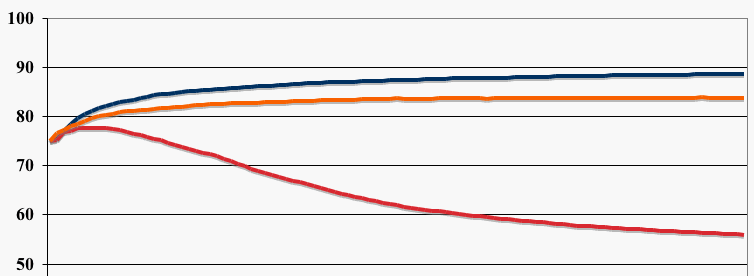
\includegraphics[width=4in]{figs/google-hire.png} 
   \caption{Comparing three hiring strategies}
   \label{fig:google_hire}
\end{figure}

Another hiring strategy we use is \textbf{no hiring manager}. Whenever you give project managers responsibility for hiring for their own projects they'll take the best candidate in the pool, even if that candidate is sub-standard for the company, because every manager wants some help for their project rather than no help. That's why we do all hiring at the company level, not the project level. First we decide which candidates are above the hiring threshold, and then we decide what projects they can best contribute to. The orange line in the graph above is a simulation of the hiring-manager strategy, with the same candidates and the same number of hires as the no-hiring-manager strategy in blue. Employees are grouped into pools of random size from 2 to 14 and the hiring manager chooses the best one. We're pleased that these little simulations show our hiring strategy is on top. 


\subsection{Internal Reference}

I would suggest that anyone who wants to apply have someone within the company refer you. For one thing they'll be able to guide you through the process better and (hopefully) set your expectations correctly.

Plus a strong internal reference will help you much more than acing an interview question.

\subsection{Personel Characters}
Personally, in my interviewing I don't care at all about schools or GPAs. (I think the only time I've even considered the school is when candidates are from a big name school like MIT, where I will modify my interview to ask more culture questions to try to see whether they are too full of themselves.)
Instead, consider this: hiring someone who isn't good is much more costly than not hiring someone who is good. It's not only that you need to pay a person who doesn't do good work, but they're also a drag on everyone else who is already really busy.

That is to say, it's much better to err on the side of "no hire" when you have any doubt; Google has plenty of employees already, and while they surely want more (and the bar is continually lowering), there's also no shortage of people who are willing to go through the legendarily Kafkaesque interview process repeatedly.
So it is possible that your one bad interview sunk you, even when it wasn't indicative of your skill. Everyone has bad days or bad luck sometimes, so don't feel too bad about it. You're in a good position in the world where there are many other tech companies eager to hire you as well and even compete on what they offer you.

It's very subjective and falls clearly in the category of "You recognize it when you see it".
Typical example of a hiring committee deliberation at Google: "He didn't find the optimal solution but he looked very excited about the problem when he was trying to solve it".
Enthusiasm, interest, being personable, excitement about solving problems, all these things count when you interview, especially at Google.
\newline

2 years isn't enough time to learn how to program. Then again, I'm not really sure you can reliably make programmers with a substantial degree of success. In my undergrad CS program, we had 300 freshman at the start, and I graduated with 29 others at the end. For people with a CS undergrad, an MS program is quite good. They shore up on depth and theory that they didn't get while working on their programming chops in undergrad.
Sadly, if you can't already program, you can get a master's in CS (because it's focused on depth and theory instead of programming), it's just completely useless. I have no idea what one can do with a MS-CS, if they can't program. It's honestly a little heartbreaking for me, that people to spend 2 years of their lives wasting it on that.
With all that said, I haven't found any degree (at least from any school I've interviewed applicants for) to be a reliable signal for programming. Even if they went to a really good school, there's a good chance that they spent all their time learning network protocols and low-level mechanisms, and will happily write up a sliding-window implementation for me, but will stare at me blankly when I ask for a simple recursive algorithm. It's just tough to find people that spent time studying and practicing general-purpose computer science.

\subsection{How to Judge an Interviewee by Answering Questions}
Starting with a basic solution won't hurt you either. You're right that staring at the whiteboard blankly for half an hour is the wrong thing to do. More than the code itself, the interviewer is interested in how you think and how you apply your knowledge to find a solution more than the solution itself. A suboptimal solution that works trumps no solution or even a more optimized solution with serious problems. It's totally fine to start with something that works and then refine.

I like to interview candidates by asking them to solve a simple programming problem and then modifying the specification little by little, having them adjust their solution to implement new functionality. There are about 8 steps in my question, and frequently I'm gauging the quality of the candidate by how long it takes him to get through the first N stages; we fix bugs in earlier stages before moving on to the next stage. To calibrate myself, I've tried this question on several of my coworkers, and they were universally able to get about halfway through the question with bug-free code in about 10 minutes. Only one required prompting on my part to fix a bug. Most every candidate I've interviewed has taken 20-30 minutes to get to the same halfway point; by that time I've only got 15-25 minutes left in my interview, and the candidate seems so far like a "no hire", so I move to a different question to find out if the candidate has other strengths to counterbalance his weakness at solving this (simple) coding problem.

From the candidate's perspective, he only sees me ask a series of programming questions which he answers satisfactorily with a little prompting from me. If he answers another question or two satisfactorily, he may think he's done well, but he doesn't know that I wanted to delve more deeply into every question I asked him, and just didn't have time because the pace of his solutions was too slow.

\subsection{The Art of Answer Questions}
For many of the questions I use during the interview process, I have a pretty good calibration level regarding how long it should take someone to answer a question. If the last couple of times I've used the question, the candidates were able to come up with an answer in 5 minutes, and then another candidate spends 10 minutes writing down an $O(n^{3})$ solution, and then tries to come up with an more optimal solution, it might be understandable why I might give that last candidate a somewhat lower score.
One thing that can help is to also keep talking so the interviewer knows what you are thinking. That way if you outline an $O(n^{2})$ solution very quickly, and then say, I think I can get a $O(n \log n)$ solution this other way, then you're showing your work, and it's a lot easier to get partial credit on a question.
In general it's better to explain the approach you want to take before you start coding. If an interviewer knows that you're going off in the weeds, perhaps because you misunderstood the problem, that will be an opportunity for the interviewer to clarify the problem, and perhaps give you a hint to steer you in the right direction. (Remember, most of the time the interviewer has used this question multiple times in the past, so s/he know where people are likely to get stuck, and very likely has hints prepared if people stumble --- and one or two stumbles does not a No Hire make; the goal is to see how someone codes and how they think, you don't get a 0 or 1 grade.)

\subsection{What to do when you fail in an interview}
As someone who was rejected by Google the first time, and hired the second time through, I went through a similar range of emotions during that first rejection. (I did not have an Ivy league education and only had a 3.2 GPA)
It was only after I was later hired into Google that I learned from my original recruiter that I had actually done quite well in my first interview process. What I did not know at the time of my rejection letter was that they had narrowed down their pool of potential applicants to about 1200 resumes for three open positions they were looking to fill. Apparently, I made it into the last round of 10-12 applicants and just did not have the experience level with the specific tools for the job as others did. Thus, I received the same rejection letter the other 1196 people received, and never even knew I did as well as I did.
My advice would be to just stay in contact and keep Google updated anytime you have something new added to your resume or skill set. Based on what you have described, it actually sounds like you might have done pretty well. There are too many factors going on behind the scenes to say one way or another why you did not make it through this time.


\end{document}